%%%%%%%%%%%%%%%%%%%%%%%%%%%%%%%%%%%%%%%%%%%%%%%%%%%%%%%%%%%%%%%%%%%%
\section{Interfaces} % (3 pages)} 
\label{sec:fdsp-apa-intfc}

The interface between the \dword{apa} consortium and other detector consortia, facilities, and working groups covers a wide range of activities. Table~\ref{tab:apa_interface_docdb} summarizes the interface control documents under development. In the following, we elaborate slightly on the interfaces with the TPC readout electronics and the \dword{pds}, as well as the connections between neighboring \dwords{apa} in the \dword{spmod} and cable routing.  Other important interfaces are to the TPC \dword{hv} system (the \dword{fc}) and the \dword{dss} inside the DUNE cryostats.  In all cases, the reader is referred to chapters within the \dword{tdr} dedicated to these systems for more information. 
\fixme{TDR or TP?}

\begin{dunetable}[\dword{apa} interface control documents]{lr}{tab:apa_interface_docdb}
{Summary of interface control documents being developed.}  
  Interface Document & DUNE doc-db number \\\hline
  Interface to TPC electronics & 6670 \\ 
  Interface to photon detector system & 6667 \\
  Interface to drift high voltage system & 6673 \\
  Interface to DAQ & 6676 \\
  Interface to slow controls and cryogenics infrastructure & 6679 \\\hline
  Integration facility interface & 7021 \\
  Facility interfaces (Detector Hall, Cryostat, and Cryogenics) & 6967 \\
  Installation interface & 6994 \\
  Calibration interface & 7048 \\\hline
  Software computing interface & 7102 \\
  Physics interface & 7075 \\
\end{dunetable}


%%%%%%%%%%%%%%%%%%%%%%%%%%%%%%%%%%%%%%%%%%%%%%%%%
\subsection{TPC Cold Electronics}
\label{sec:fdsp-apa-intfc-elec}

The TPC readout electronics is directly mounted to the \dword{apa} immersed in \lar in order to reduce the input capacitance and thus the inherent electronics noise.  With the wire-wrapped design, all \num{2560} wires to be read out (recall \num{960} are $G$-plane wires used for charge shielding only and so not read out) are terminated on wire boards that stack along one end (the head) of the \dword{apa} frame.  The \num{2560} channels are read out by \num{20} \dword{fe} motherboards (\num{128} channels per board), each of which includes eight \num{16}-channel \dword{fe} ASICs, eight \num{16}-channel ADC ASICs, low-voltage regulators, and input signal protection circuits.  A schematic view of the head end of an \dword{apa} with electronics installed and a cable tray mounted above is shown in Figure~\ref{fig:apa_ce}. 

\begin{dunefigure}[\dword{apa} interface with TPC electronics]{fig:apa_ce}
{The head region of an \dword{apa} frame showing the 10 wire board stacks on each side, \num{20} \dword{fe} motherboard boxes, and the cable tray mounted above.}
%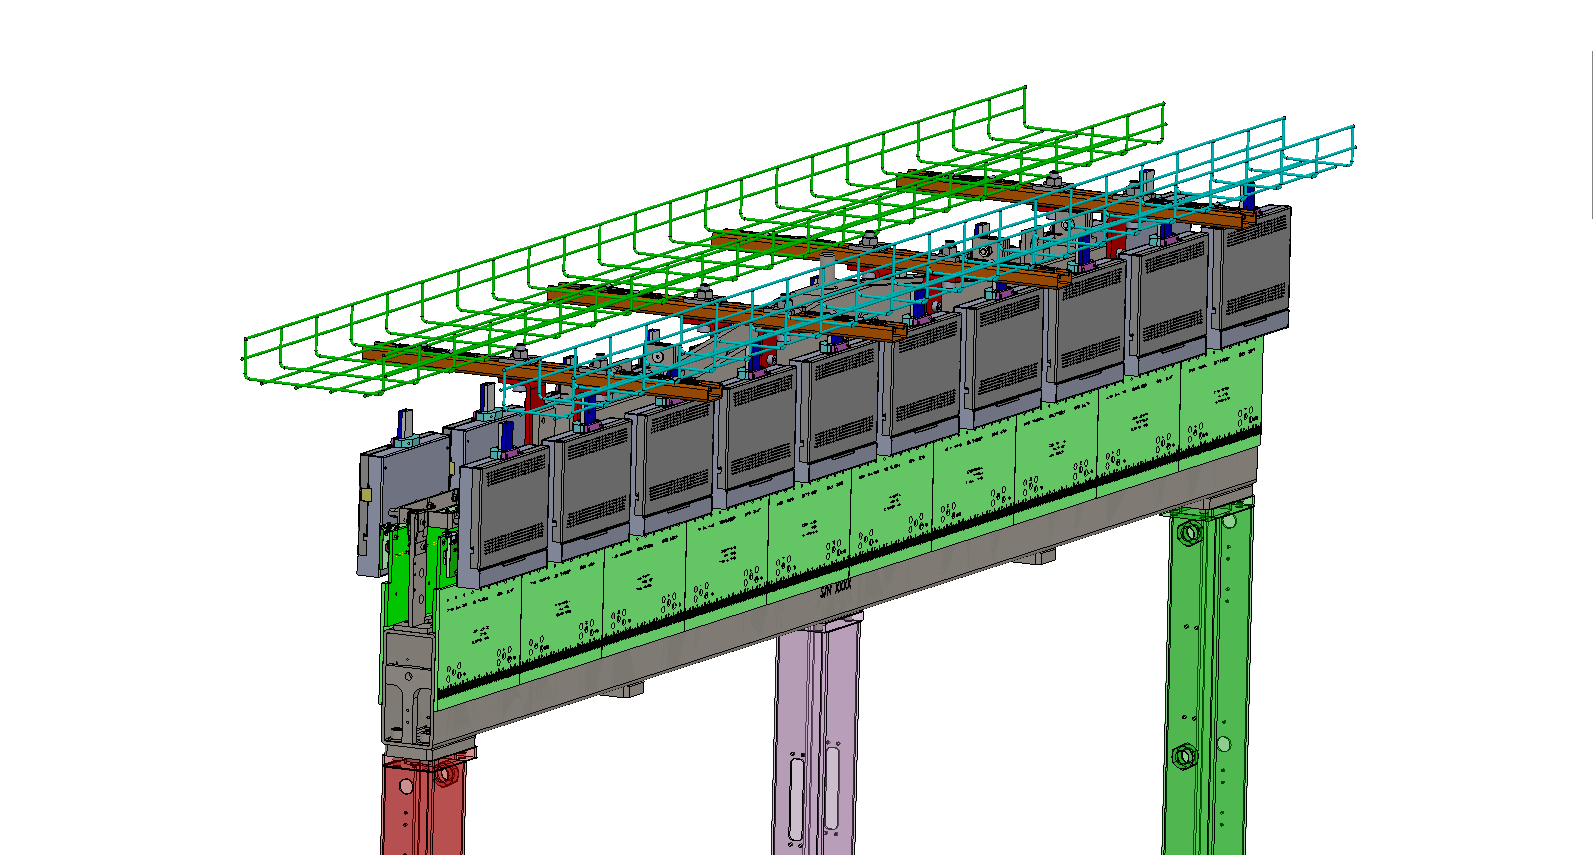
\includegraphics[width=0.85\textwidth,trim=10mm 0mm 10mm 20mm, clip]{apa-elec-interface.png}
\end{dunefigure}

The interface between the \dword{apa} and TPC \dword{ce} covers a wide range of topics, including the hardware design and production, testing, integration, installation, and commissioning. The hardware interface has two basic components, mechanical and electrical. The mechanical interface includes the support of the \num{20} \dword{ce} boxes with each housing a \num{128} channel \dword{fe} motherboard.  These are the gray colored, vertically oriented boxes shown in Figure~\ref{fig:apa_ce}. 

The electrical interface covers the choice of wire-bias voltages to the four wire planes so that \num{100}\% transparency can be achieved for drifting ionization electrons, cable connection for the wire bias voltages from the cryostat feedthroughs to the CR boards, interface boards providing connection between CR boards and \dword{ce} boxes, filtering of the wire-bias voltages through CR boards in order to suppress potential introduction of electronics noise, and an overall grounding scheme and electrical isolation scheme for each \dword{apa}. The last item is particularly important in order to reach the low electronics noise levels required.  See Chapter~\ref{ch:fdsp-tpc-elec} for information on all of these aspects of the \dword{fe} electronics system.


%%%%%%%%%%%%%%%%%%%%%%%%%%%%%%%%%
\subsection{Photon Detection System}
\label{sec:fdsp-apa-intfc-pds}

While the design of the \dword{pds} is still under development, it is expected that it is integrated into the \dword{apa} frame to form a single unit for the detection of both ionization charge and scintillation light.  Cables for the \dwords{pd} must also be accommodated in the \dword{apa} frame design.  Figure~\ref{fig:apa-pd} shows the interface for a light-guide bar based \dword{pds} as has been deployed in \dword{pdsp}. Individual bars were inserted through \num{10} slots left on the side steel tubes of the frame. Rails mounted in the \dword{apa} frame, as shown in Figure~\ref{fig:apa-frame-2}, support the bars in their final positions. 

\begin{dunefigure}[\dword{apa} interface with \dwords{pd} in \dword{pdsp}]{fig:apa-pd}
{Installation of a light-guide bar photon detector module into the available slots in the \dword{apa} frame. Also shown is a concept for routing \dword{pds} cables through the rib tubes of the \dword{apa} frame and up the central vertical tube section.}
%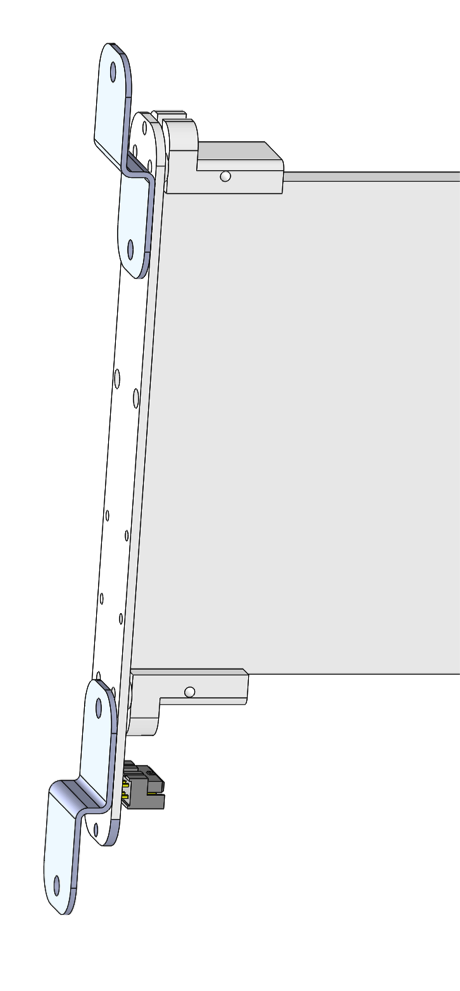
\includegraphics[height=0.3\textheight]{apa-light-bar-detail.png}\qquad\qquad
%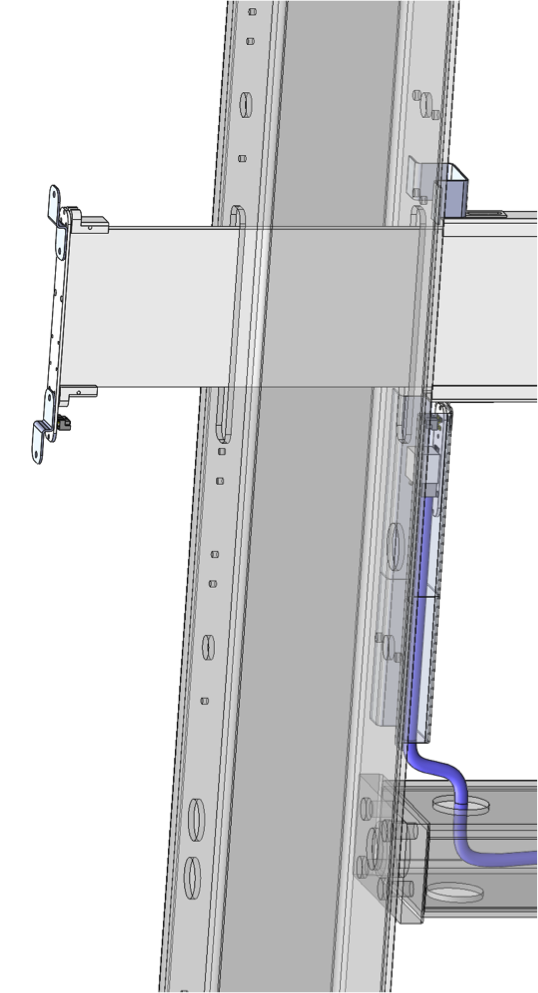
\includegraphics[height=0.3\textheight]{apa-light-bar-insert.png}\qquad\qquad
%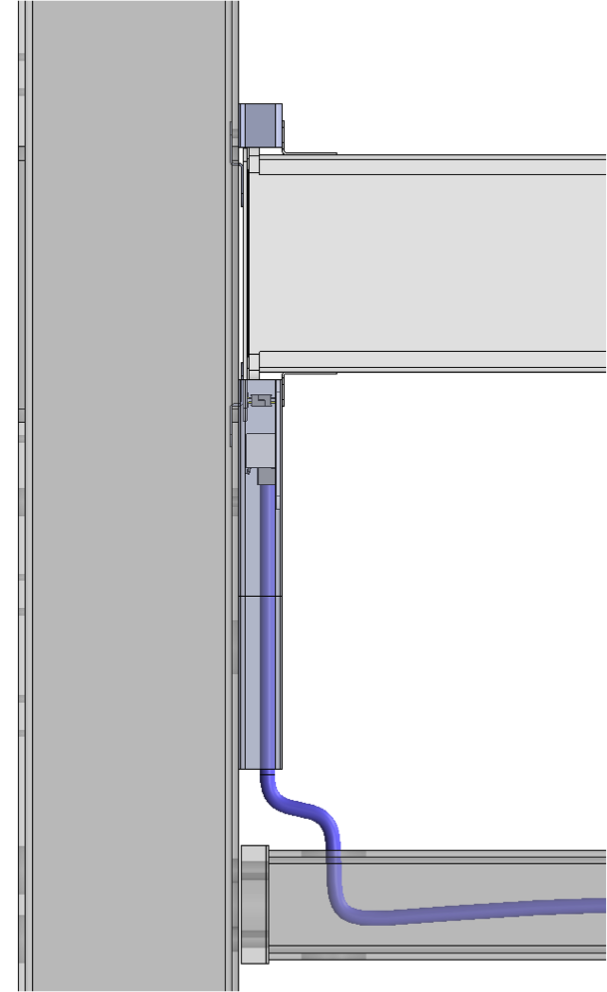
\includegraphics[height=0.3\textheight]{apa-light-bar-cable.png}
\end{dunefigure}

Similar to that of the \dword{ce}, the interface between the \dword{pds} and \dwords{apa} covers a wide range of topics, including the hardware design and production, testing, integration, installation, and commissioning. Depending on the final design of the \dword{pds}, the geometry of the \dword{apa}, including access slot dimensions, locations, and number, may require modification. Any proposed changes by the \dword{pds} consortium must be evaluated by the \dword{apa} consortium to understand structural impacts or interferences with other components.  The electrical interface includes a grounding scheme and electrical insulation. Due to the strict requirements on the noise from the \dword{ce}, the electrical interface must be defined together with the \single electronics consortium. 

For more information on the photon system, see Chapter~\ref{ch:fdsp-pd} % the Photon Detector Chapter in the \dword{tdr}.


%%%%%%%%%%%%%%%%%%%%%%%%%%%%%%%%%
\subsection{\dword{apa} to \dword{apa} Connections and Cable Routing}
\label{sec:fdsp-apa-intfc-apa}

The TPC readout electronics require that the \dword{apa} frames must be electrically isolated.  The left panel of Figure~\ref{fig:apa-cabling} shows the current conceptual design for mechanically connecting the two \dwords{apa} in a vertical stack while maintaining electrical isolation.  The green elements are an insulating panel and bolt sleeve made from G10. 

Cable routing schemes for both the TPC electronics and \dword{pds} are actively being developed.  A concept currently under evaluation is to run the cables of the \dword{pds} inside the crossing rib tubes to the central beam tube of the \dword{apa} frames to get to the top.  The \dword{ce} signal and power cables also need to be routed so that the head end of the lower \dword{apa} in the 2-\dword{apa} assembly can be reached. The current concept is to route the electronics cables inside the two side beams of the \dword{apa} frames. The right panel of Figure~\ref{fig:apa-cabling} depicts such a cable routing scheme. To fully accommodate the cables from two \dwords{apa}, it is being considered to modify the \dword{apa} frame design to use larger hollow tube sections. The final design is in progress and prototyping is planned for later this year to verify a cabling and installation solution.     

\begin{dunefigure}[\dword{apa}-to-\dword{apa} connection and cable routing]{fig:apa-cabling}
{Left: Conceptual design for the \dword{apa}-to-\dword{apa} connection.  The green insulator pieces act to electrically isolate the two frames, as required by the \dword{fe} electronics.  Right: A concept for TPC electronics and \dword{pds} cable routing. Photon detector cables would go through the central beam and be distributed inside the supporting tubes of the \dword{apa} frame.  \Dword{ce} cables (both data and power) from the bottom \dword{apa} electronics would go through the outside tubes to reach the top of the stack.}
\setlength{\fboxsep}{0pt}
\setlength{\fboxrule}{0.5pt}
%\fbox{%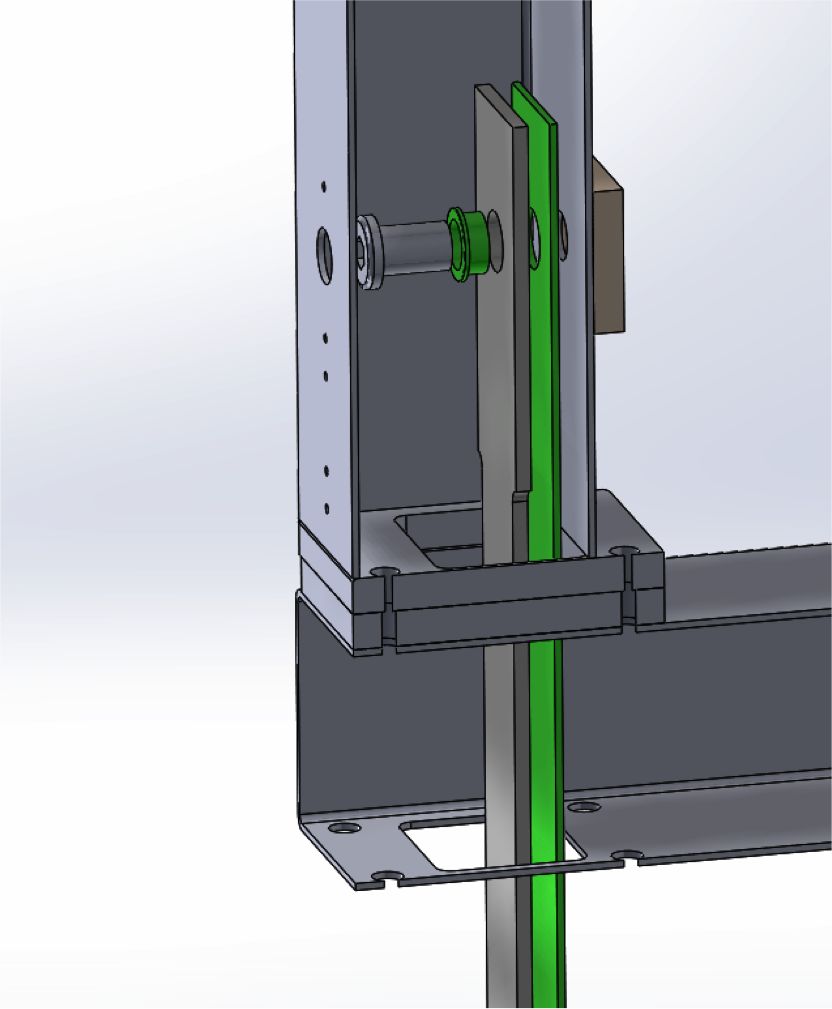
\includegraphics[height=0.26\textheight]{apa-apa-mating.png}}\qquad \quad
%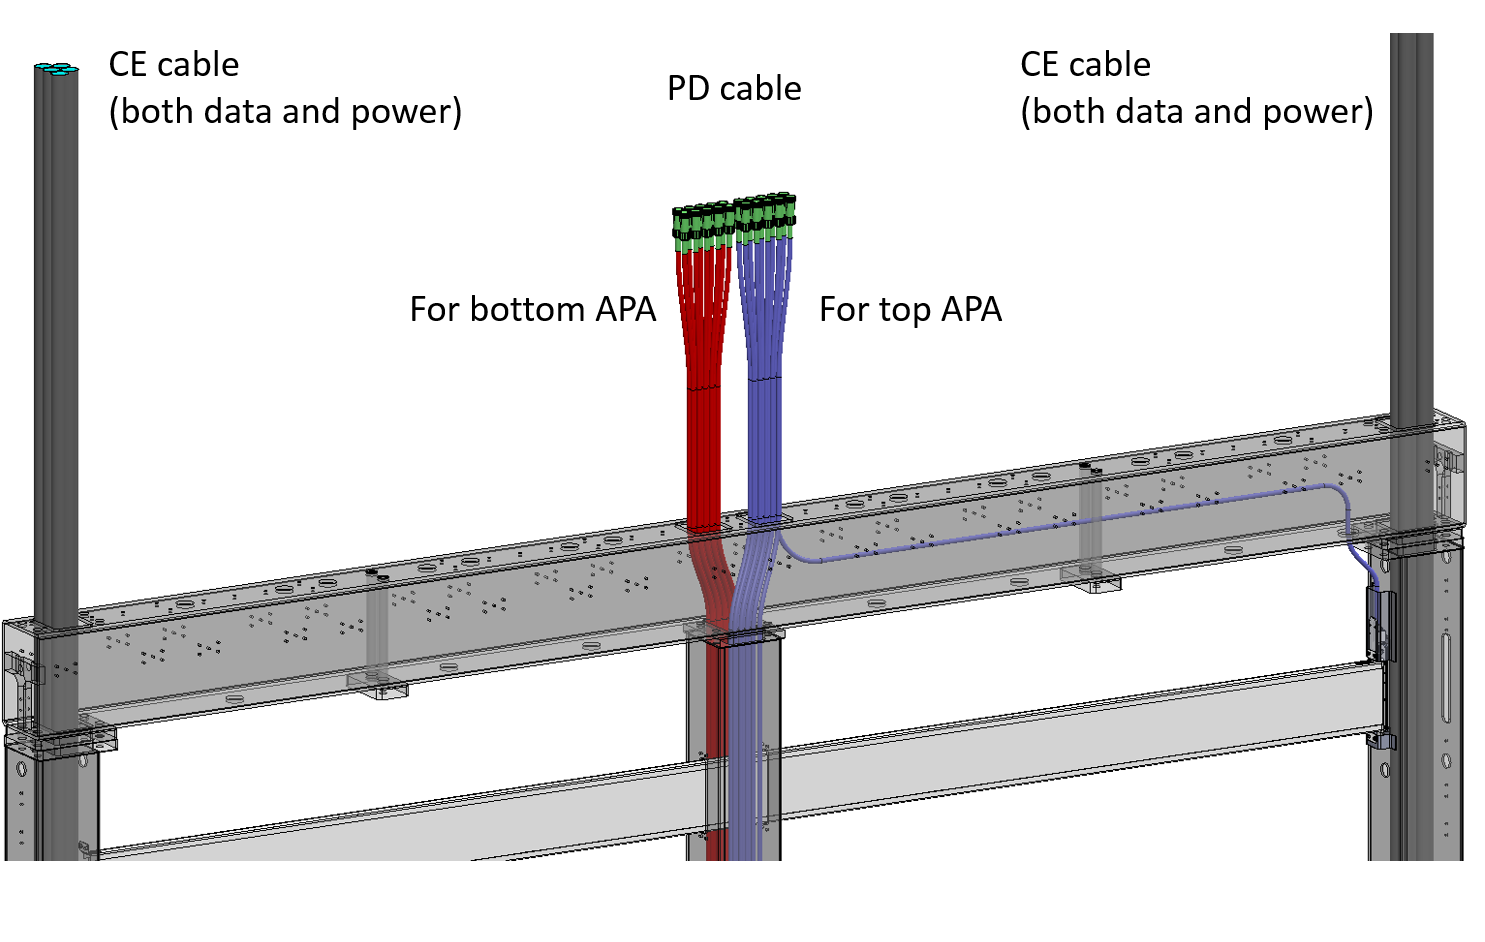
\includegraphics[height=0.26\textheight]{apa-cable-routing.png}
\end{dunefigure}
